%! TEX root = ../000-main.tex
\chapter[Multiple non-parametric regression]{Multiple (generalized) non-parametric regression}
\chaptermark{M NP reg.}

The extension of the non-parametric regression model to the case in which there are
$p$ explanatory variables is straightforward:
\begin{equation*}
    y_i = m(x_{i1}, \ldots, x_{ip}) + \varepsilon_i, \quad i = 1, \ldots, n.
\end{equation*}
with $\mathds E(\varepsilon_i) = 0$ and $\text{Var}(\epsilon_i) = \sigma^2$.

The regression function $m$ indicates how $y$ varies depending on the
$p$-dimensional explanatory variable $\boldsymbol x = (x_1, \ldots, x_p)$.

\section{Local polynomials}
To define the \iemph{local polynomial estimator} of the regression function $m$
we need both to define the weights $w_i$ for each observation and to specify
which explanatory variables are included at each local linear regression model.

\subsection{Defining the weights}

When estimating $m(\boldsymbol t)$ with $\boldsymbol t = (t_1, \ldots, t_p)$,
data $(y_i;\,x_{i1}, \ldots, x_{ip})$ with $\boldsymbol x_i = (x_{i1}, \ldots, x_{ip})$
closer to $\boldsymbol t$ should have greater weight than those
data that are further.

Now distances between $\boldsymbol t$ and $\boldsymbol x_i$ are measured in
a $p$-dimensional space and there are many sensible ways to define distances in 
such a space.

\begin{definition}{Weights for local polynomials in multiple non-parametric regression}{}

A way to define weights $w_i$ with good performance in practice is:
\begin{equation*}
    w_i = w(\boldsymbol t,\, \boldsymbol x_i) \propto \pi_{j=1}^p
    K\left(\frac{t_j - x_{ij}}{h_j}\right)
\end{equation*}
where $K$ is a univariate kernel function and $h_j$ is a smoothing parameter
well suited for variable $j$-th.
\end{definition}

\subsection{Explanatory variables at each local linear model}

To fit a degree $q$ polynomial depending on $p$-variables, all possible terms with the form:
\begin{equation*}
    \beta_{s_1, \ldots, s_p} \prod_{j=1}^p \left(
        x_{ij} - t_j
    \right)^{s_j}
\end{equation*}
with degree $\sum_{j=1}^p s_j \leq q$ must be included.

The estimate of $m(\boldsymbol t)$ will be the intercept of the local polynomial
fitted around point $\boldsymbol t$: $\hat m(\boldsymbol t) = \hat m(t_1, \ldots, t_p) = \hat \beta_{0\cdots 0}$.

\begin{example}{Two explanatory variables, local polynomial with degree 2}{}
    \begin{equation*}
        \beta_{00} + \beta_{10} (x_{i1} - t_1)
        + \beta_{01} (x_{i2} - t_2)
        + \beta_{11} (x_{i1} - t_1)(x_{i2} - t_2)
        + \beta_{20} (x_{i1} - t_1)^2
        + \beta_{02} (x_{i2} - t_2)^2
    \end{equation*}
    \tcblower
    The estimate of $m$ at $\boldsymbol t = (t_1, t_2)$ will be $\beta_{00}$.
\end{example}

\begin{example}{Boston housing data bivariate regression}{boston1}
    Non-parametric fit of \texttt{ROOM} as a function of \texttt{LSTAT}
    and \texttt{AGE}.

    We use a kernel product of two univariate Gaussian kernels with
    smoothing parameters $h_{LSTAT} = 2.85$ and $h_{AGE} = 10$:

    \begin{figure}[H]
        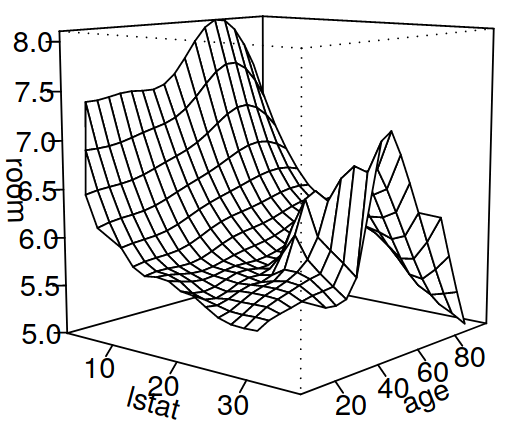
\includegraphics[width=0.6\textwidth]{boston_bivariate}
        \caption{Non-parametric fit of \texttt{ROOM} as a function of \texttt{LSTAT} and \texttt{AGE}.}
    \end{figure}
\end{example}

\pagebreak
\section{Splines}

Smoothing splines can be generalized to higher dimensions:
\begin{problem}{Smoothing splines for higher dimensions}{}
    \begin{equation*}
        \min_{\tilde m} \sum_{i=1}^n  \left( y_i - \tilde m*\boldsymbol x \right)^2 + \lambda \phi (\tilde m)
    \end{equation*}
    where (assuming that there are only $p=2$ predictors):
    \begin{equation*}
        \phi(f) = \mathlarger{\int} \int_{\mathbb R^2}
            \left( \frac{\partial^2 f(x_1, x_2)}{\partial x_1^2} \right)^2
            + 2 \left( \frac{\partial^2 f(x_1, x_2)}{\partial x_1 \partial x_2} \right)^2
            + \left( \frac{\partial^2 f(x_1, x_2)}{\partial x_2^2} \right)^2
            \, dx_1 \, dx_2
    \end{equation*}
    \tcblower
    The solution is a \iemph{thin plate spline}, a function of the form (for $p=2$):
    \begin{equation*}
        \tilde m (\boldsymbol x) = \beta_0 + \boldsymbol\beta^T \boldsymbol x
        + \sum_{i=1}^n \alpha_jh_i(\boldsymbol x)
    \end{equation*}
    where $h_i(\boldsymbol x) = \eta \left( \lVert \boldsymbol x - \boldsymbol x_i \rVert \right)$
    and $\eta(z) = z^2 \log(z)$.

    Basis is: $\{h_i(\boldsymbol x)\}_{i=1}^n$: as many elements as observations.

    \begin{note}
        High computational complexity: $O(n^3)$ for $p \geq 2$. Approximations
        with complexity $O(pn^2)$ are possible. We can reduce the number of
        knots.
    \end{note}
\end{problem}

\subsection{Tensor product splines}
Consider the case of $p=2$ explanatory variables $x$ and $z$.

Assume that basis of functions for expanding univariate functions depending on either
$x$ or $z$, have been determined:
\begin{equation*}
    f_X(x) = \sum_{j=1}^J \alpha_ja_j(x),\quad f_Z(z) = \sum_{h=1}^H \beta_hb_h(z)
\end{equation*}

Then, a \iemph{tensor product basis} for functions depending on both $x$ and $z$ is
defined as the collection of:
\begin{equation*}
    \left\{
        a_j(x) b_h(z) \mid j=1,\ldots,J,\, h=1,\ldots,H
    \right\}
\end{equation*}
that allows for expansions of the form:
\begin{equation*}
    f(x,z) = \mathlarger{\sum_{j=1}^J} \sum_{h=1}^H \gamma_{jh} a_j(x) b_h(z)
\end{equation*}

\begin{figure}[H]
    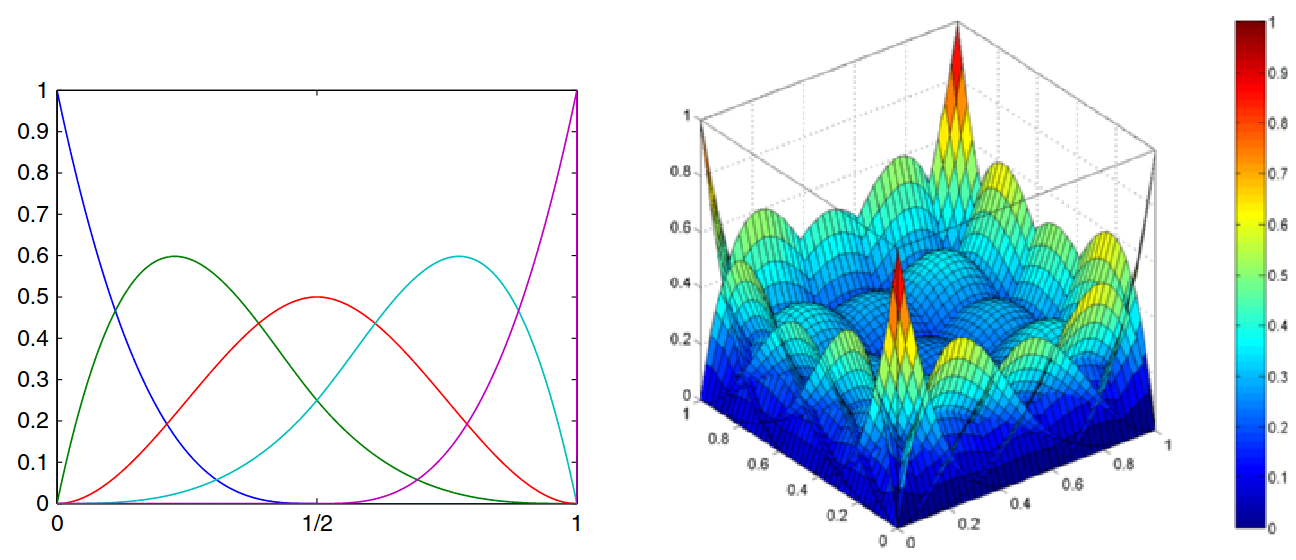
\includegraphics{2d_cubic_bsplines}
    \caption{1D and 2D cubic B-splines basis functions.}
    % https://www.researchgate.net/publication/270665031_Upper_bound_limit_analysis_of_plates_using_a_rotation-free_isogeometric_approach
\end{figure}

Fitting functions:
\begin{equation*}
    f(x,\,z) = \mathlarger{\sum_{j=1}^J} \sum_{h=1}^H \gamma_{jh} a_j(x) b_h(z) = \boldsymbol g(x,\,z)^T \boldsymbol\gamma
\end{equation*}

Penalty for tensor product splines (two penalty parameters):
\begin{align*}
    \phi(f) &= \mathlarger{\int} \int_{\mathbb R^2}
    \lambda_x \left( \frac{\partial^2 f(x,\,z)}{\partial x^2} \right)^2
    + \lambda_z \left( \frac{\partial^2 f(x,\,z)}{\partial z^2} \right)^2
    \, dx \, dz \\
            &= \lambda_x \boldsymbol \gamma^T \boldsymbol D_x \boldsymbol \gamma
            + \lambda_z \boldsymbol \gamma^T \boldsymbol D_z \boldsymbol \gamma
\end{align*}

\begin{problem}{Tensor product splines (p = 2)}{}
    \begin{equation*}
        \min_{\boldsymbol \gamma \in \mathds R^{J \times H}}
        \left(
            Y - \boldsymbol G\boldsymbol \gamma
        \right)^T
        \left(
            Y - \boldsymbol G\boldsymbol \gamma
        \right)
        + \lambda_x \boldsymbol \gamma^T \boldsymbol D_x \boldsymbol \gamma
        + \lambda_z \boldsymbol \gamma^T \boldsymbol D_z \boldsymbol \gamma
    \end{equation*}
    \tcblower
    \begin{note}
        \paragraph{Main drawback:} Exponential growth in basis functions as $p$ increases.
        So, we must reduce the number of basis per coordinate.
    \end{note}
\end{problem}

\pagebreak
\section{The curse of dimensionality}\index{curse of dimensionality}

Recall the problem introduced in \cref{sec:curse-of-dimensionality}. As explained
there, non-parametric estimation of the regression function is extremely difficult
when $p$ is large ($p \geq 4$). One way to solve this problem
is to use \emph{extremely} large sample sizes, (note that
for some problems having 842,000 observations in 10 dimensions is
equivalent to having 4 observations in 1 dimension).

For an exploratory variable in $\mathds R^p$, it can be proved that
the linear regression has $\text{AMSE}_0 = O(n^{-4/(p+4)})$.

The higher the dimension $p$ of explanatory variable, the lower the precision with which
the regression function is estimated.

There exist proposals, alternative to local polynomial regression or spline smoothing,
that overcome the curse of dimensionality:
Additive models and Projection pursuit are two of them that will be discussed in the
following sections.

\pagebreak
\section{Additive Models}

\begin{definition}{Additive Model}{additive-model}\index{additive model}
    \begin{equation*}
        y_i = \alpha + \sum_{j=1}^p g_j(x_{ij}) + \epsilon_i
    \end{equation*}
    where $\mathds E(\epsilon_i) = 0$, $\text{Var}(\epsilon_i) = \sigma^2$ and
    $\mathds E(g_j(X_{j})) = 0$.

    Functions $g_j$ are called \iemph{additive components} and must be estimated
    non-parametrically because no parametric model is specified for them.

    \tcblower

    The main assumption in this model is that the non-parametric univariate functions
    $g_j$ are combined additively to produce the non-parametric $p$-dimensional
    regression function.

    \begin{note}
        The additive model is halfway between the multiple linear regression model
        (which additively combines linear transformations of the explanatory variables: $\beta_jx_{ij}$)
        and the multiple non-parametric regression model.
    \end{note}
\end{definition}

\begin{example}{Boston housing data additive model}{}
    This is the same as in example~\ref{ex:boston1}, but using an additive model.
    \begin{figure}[H]
        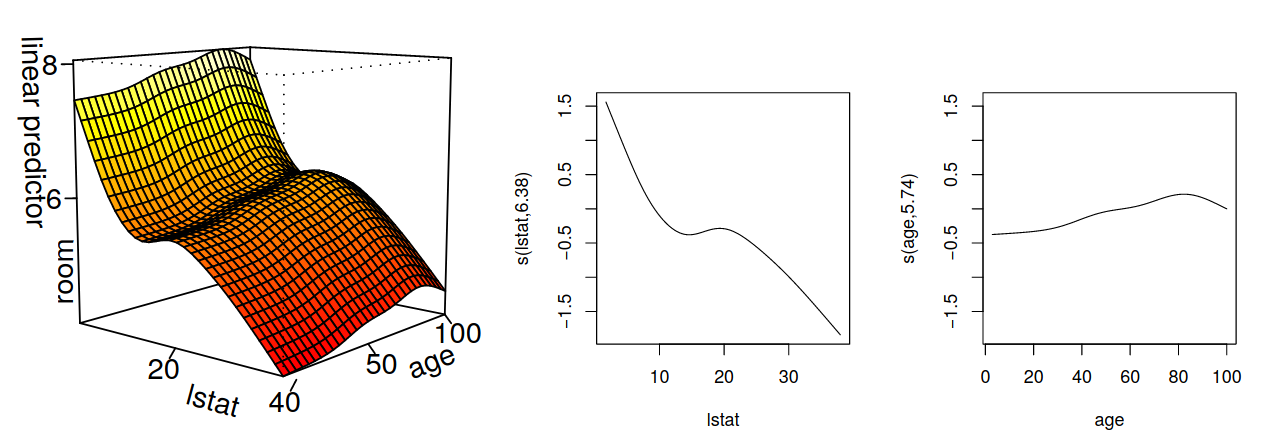
\includegraphics{additive}
        \caption{Non-parametric additive model of \texttt{ROOM} as a function of \texttt{LSTAT} and \texttt{AGE}.}
    \end{figure}

    \tcblower

    If we compare this model with the bivariate one, we can see that the additive model
    cannot pick up the local maximum located around $(\texttt{LSTAT},\, \texttt{AGE}) = (35,\, 50)$ because
    it is more rigid than the non-parametric bivariate model.

    \begin{note}
        The surface can be obtained by shifting the function $g_{LSTAT}$ over the function
        $g_{AGE}$ or vice versa and adding the mean of \texttt{ROOM}.
    \end{note}
\end{example}

\pagebreak
\subsection{Estimating the additive model}
Observe that $\mathds{E}(y_i) = \alpha$ since $\mathds{E}(\epsilon_i) = 0$
and $\mathds{E}(g_j(X_{j})) = 0$ (see~\ref{def:additive-model}).

Assume for a moment that the parameter $\alpha$ and all functions
$g_j$ are known except for $g_k$. Then $g_k$ could be estimated using
a non-parametric univariate smoother (i.e. local linear fit).
It would be enough to apply the smoother to data $(x_{ik},\, y_i^{(k)})$
where:
\begin{equation*}
    y_i^{(k)} = y_i - \alpha - \sum_{j \neq k} g_j(x_{ij})
\end{equation*}

This reasoning leads to the \iemph{backfitting} algorithm to estimate
the additive model.

\begin{algorithm}{Backfitting algorithm}{backfitting}
    \begin{enumerate}
        \item Estimate $\alpha$ using the sample mean of $y_i$: $\hat \alpha = \frac{1}{n} \sum_{i=1}^n y_i$.
        \item Take an arbitrary function $\hat g_k = g_k^0$ as initial estimate of function $g_k$,
            for $k = 1,\dots,p$. (For instance, $g_k^0(x_{ik}) = \hat \beta_k x_{ik}$ where
            the coefficients $\hat \beta_k$ are estimated using the multiple linear regression model.)
        \item For $k = 1,\dots,p$:
            \begin{enumerate}
                \item Estimate $g_k$ using a non-parametric univariate smoother
                    to data $(x_{ik},\, y_i^{(k)})$ where:
                    \begin{equation*}
                        y_i^{(k)} = y_i - \alpha - \sum_{j \neq k} g_j(x_{ij})
                    \end{equation*}
            \end{enumerate}
        \item Repeat step 3 until convergence.
    \end{enumerate}
\end{algorithm}

\subsubsection{Basis functions}

Consider now the expansion of each function $g_j(x_j)$ in a basis function
(B-splines, for instance):
\begin{align*}
    m(\boldsymbol x) &= \alpha + \mathlarger{\sum_{j=1}^p} \sum_{h=1}^H \beta_j^h b_j^h(x_j) \\
        &= \alpha + \left(
            \boldsymbol b_1(x_1)^T, \ldots, \boldsymbol b_p(x_p)^T
        \right) \begin{pmatrix}
            \beta_1 \\
            \vdots \\
            \beta_p
        \end{pmatrix}
\end{align*}

Penalty term:
\begin{equation*}
    \Psi(m) = \sum_{j=1}^p \lambda_j \int_{\mathds R} \left( g_j'' (x_j) \right) dx_j
        = \sum_{j=1}^p \lambda_j \boldsymbol\beta_j^T \boldsymbol D_j \boldsymbol\beta_j
\end{equation*}

The, the GAM model is estimated as a penalized multiple linear regression model with
$1 + \sum_{j=1}^p H_j$ parameters.

The smoothing parameters $\lambda_1,\dots,\lambda_p$ are estimated using cross-validation
(LOOCV of GCV).

\section{Generalized Additive Models}

\begin{definition}{Generalized additive models (GAM)}{GAM}\index{generalized additive model}\index{GAM}
    Additive models can be generalized similarly to generalized linear models
    (as seen in \ref{def:gnprm})

The r.v. $(Y; \boldsymbol X)$, with $\boldsymbol X = (X_1,\dots,X_p)$ has a distribution such
that:
\begin{equation*}
    (Y \mid \boldsymbol X) = (x_1,\dots,x_p) \sim f(y;\,m(x_1, \ldots, x_p),\,\psi)
\end{equation*}
where $m(x_1, \ldots, x_p) = \mathds{E}(Y \mid \boldsymbol X = (x_1,\dots,x_p))$ is a
smooth function of $(x_1,\dots,x_p)$ possible subject to certain constrains (e.g. non-negativity)
and $\psi$ represents other parameters (e.g. variance) not depending on $(x_1,\dots,x_p)$.

There exists an invertible \iemph{link function} $g$ such that:
\begin{equation*}
    \theta(x_1,\ldots,x_p) = g(m(x_1,\ldots,x_p)), \quad m(x_1,\ldots,x_p) = g^{-1}(\theta(x_1,\ldots,x_p))
\end{equation*}
where $\theta(x_1,\ldots,x_p)$ is a \iemph{smooth function} of $(x_1,\ldots,x_p)$ free of
constraints.
\tcblower
Alternatively, we can write:
\begin{equation*}
    (Y \mid \boldsymbol X = (x_1,\dots,x_p)) \sim f_2(y;\,\theta(x_1, \ldots, x_p),\,\psi)
    = f(y;\,g^{-1}(\theta(x_1, \ldots, x_p)),\,\psi)
\end{equation*}
\end{definition}

The non-parametric estimation of $\theta$ and $m$ by maximum local
likelihood suffers the effects of the \iemph{curse of dimensionality}.

A penalized maximum likelihood approach (with penalization for the
lack of smoothness of the estimated function) is also problematic
for moderate or large dimension $p$.

The possible solution is to use the \emph{Generalized Additive Model} (GAM):
\begin{equation*}
    \theta(x_1,\ldots,x_p) = \alpha + \sum_{j=1}^p g_j(x_j)
\end{equation*}

If the restriction that the functions $g_j$ are linear is added,
we obtain the \emph{Generalized Linear Model} (GLM).

\begin{note}
The GAM is halfway between the Generalized non-parametric multiple regression model
and the Generalized Linear Model.
\end{note}

\subsection{Generalized Additive Models Estimation}

The estimation of GAMs combines methods used to fit additive models with the
\iemph{IRWLS} algorithm (used to fit generalized linear models).

We replace each multiple linear regression fit by WLS is replaced
by the fitting of a weighted additive model (using backfitting
or penalized multiple linear regression, after a basis expansion)

This way, the final model is GAM instead of a GLM.

\subsection{Local scoring algorithm for logistic GAM}

\begin{algorithm}{Local scoring algorithm for logistic GAM}{LSAGAM}
\begin{enumerate}
    \item Compute starting values $\hat \alpha = \log \left( \frac{\bar y}{1-\bar y} \right)$
        where $\bar y$ is the sample proportion of ones, and set $\hat f_j = 0,\,\forall j$.
    \item Define $\hat \eta_i = \hat \alpha + \sum_{j=1}^p \hat f_j(x_{ij})$ and
        $\hat p_i = \frac{e^{\hat \eta_i}}{1+e^{\hat \eta_i}}$.
    Then Iterate:
        \begin{enumerate}
            \item Construct the working target variable $z_i = \hat \eta_i + \frac{y_i - \hat p_i}{\hat p_i(1-\hat p_i)}$.
            \item Construct weights $w_i = \hat p_i(1-\hat p_i)$.
            \item Fit a weighted additive model to the targets $z_i$ with
                exploratory variables $x_{ij}$ and weights $w_i$ using
                a weighted backfitting algorithm (or penalized basis expansions).

                This gives new estimates $\hat f_j,\,\forall j$.
        \end{enumerate}
        \item Repeat step 2 until the change in functions falls below a previously
            specified threshold.
\end{enumerate}
\end{algorithm}

\pagebreak
\section{Semi-parametric models}

Sometimes some of the explanatory variables involved in the
definition of an additive model (or GAM)
affect the response variables linearly.

If this is known in advance, the GAM model can be reformulated
allowing some functions $g_j$ to be linear:
$g_j(x_j) = \beta_j x_j$.

Other possible modifications of the GAM model are:
\begin{itemize}
    \item non-parametrically estimating the combined effect of two (or more)
        explanatory variables. This includes for examples, replacing
        $g_j(x_j) + g_k(x_k)$ by $g_{jk}(x_j, x_k)$.
    \item Estimating the effect of a variable $x_j$ differently at each of the
        classes determined by another categorical variable $x_h$. There
        effects could be estimated linearly or non-parametrically.
\end{itemize}

Models incorporating this modifications to the GAM model are known as
\iemph{semi-parametric models}.

\subsection{Software}

These models can be fitted using the function \texttt{gam} in the R package
\texttt{mgcv}. The \texttt{anova.gam} functions allows for testing between
nested GAM models.
